\documentclass[11pt,a4paper]{article}

\usepackage[utf8x]{inputenc}   % omogoča uporabo slovenskih črk kodiranih v formatu UTF-8
\usepackage[slovene]{babel}    % naloži, med drugim, slovenske delilne vzorce
\usepackage{url}
\usepackage{graphicx}



\title{Asistent Slivko \\
\large Seminarska naloga za Elektronsko in mobilno poslovanje}
\author{
Jernej Habjan, 63150106  \\
Matic Vrtačnik, 63150317 \\
\ \\
Fakulteta za računalništvo in informatiko Univerze v Ljubljani
\date{\today}         
}


\begin{document}
\maketitle


\section{Zgradba aplikacije}

Okna pri aplikaciji so fragmenti, ki so povezani preko glavne aktivnosti, skozi katero si izmenjujejo podatke.
Aplikacija ima poleg pomikanja skozi okna z gumbi tudi navigacijsko okno, s katerim se lahko vrnemo na različne zaslone, pri vnašanju potnikov in informacij o letu nas pa aplikacija sama vodi skoz njih.
Komunikacija med fragmenti poteka z Bundle preko Vmesnikov, ki jih implementira glavna aktivnost


\section{Storitve}
Aplikacija ima 3 storitve:
\begin{itemize}
	\item Google Login~\cite{signIn} - S katerim se lahko prijavimo v aplikacijo z Googlovim računom.
	\item Google Autocomplete\cite{autocomplete} - Polje ki se samo izpolnjuje, ko pišemo vanj kraje. Ista funkcionalnost kot vnosno polje na Google Maps.
	\item REST storitev za upravljanje podatkovne baze na Microsoft Azure.
\end{itemize}


\section{Podatkovna baza}
S podatkovno bazo, ki je dostopna na portalu Microsoft Azure, upravljamo preko REST storitev.
Storitve kličemo z odjemalca android z uporabo knjižnice Volley (Pokrite vse CRUD zahteve)
\begin{itemize}
	\item Za registracijo uporabnika z Googlovim ID v lastno podatkovno bazo,
	\item Pridobitev informacij o uporabniku iz baze,
	\item Vnos in pridobitev informacij o naročilu, letu, letalu in potnikih v in iz baze,
	\item Preimenovanje uporabniškega imena,
	\item Izbris prejšnih potovanj

\end{itemize}

\section{Gradnja aplikacije}

Aplikacija je bila že delno izgrajena za predmet Uporabniški vmesniki, kjer so bili ustvarjeni osnovni fragmenti in njihova komunikacija.
Za implementacijo Google Sign-In sva si pomagala z s predlogo, objavljeno na Google GitHub repozitoriju, ki vsebuje primer fragmenta z implementirano prijavo~\cite{loginSample}.
Prav tako sva si veliko pomagala s stranjo Stack Oveflow za razreševanje problemov~\cite{stack}.
Aplikacija je izdelana v programskem jeziku Kotlin.

\section{Slike}

\begin{figure}[htb]
\centerline{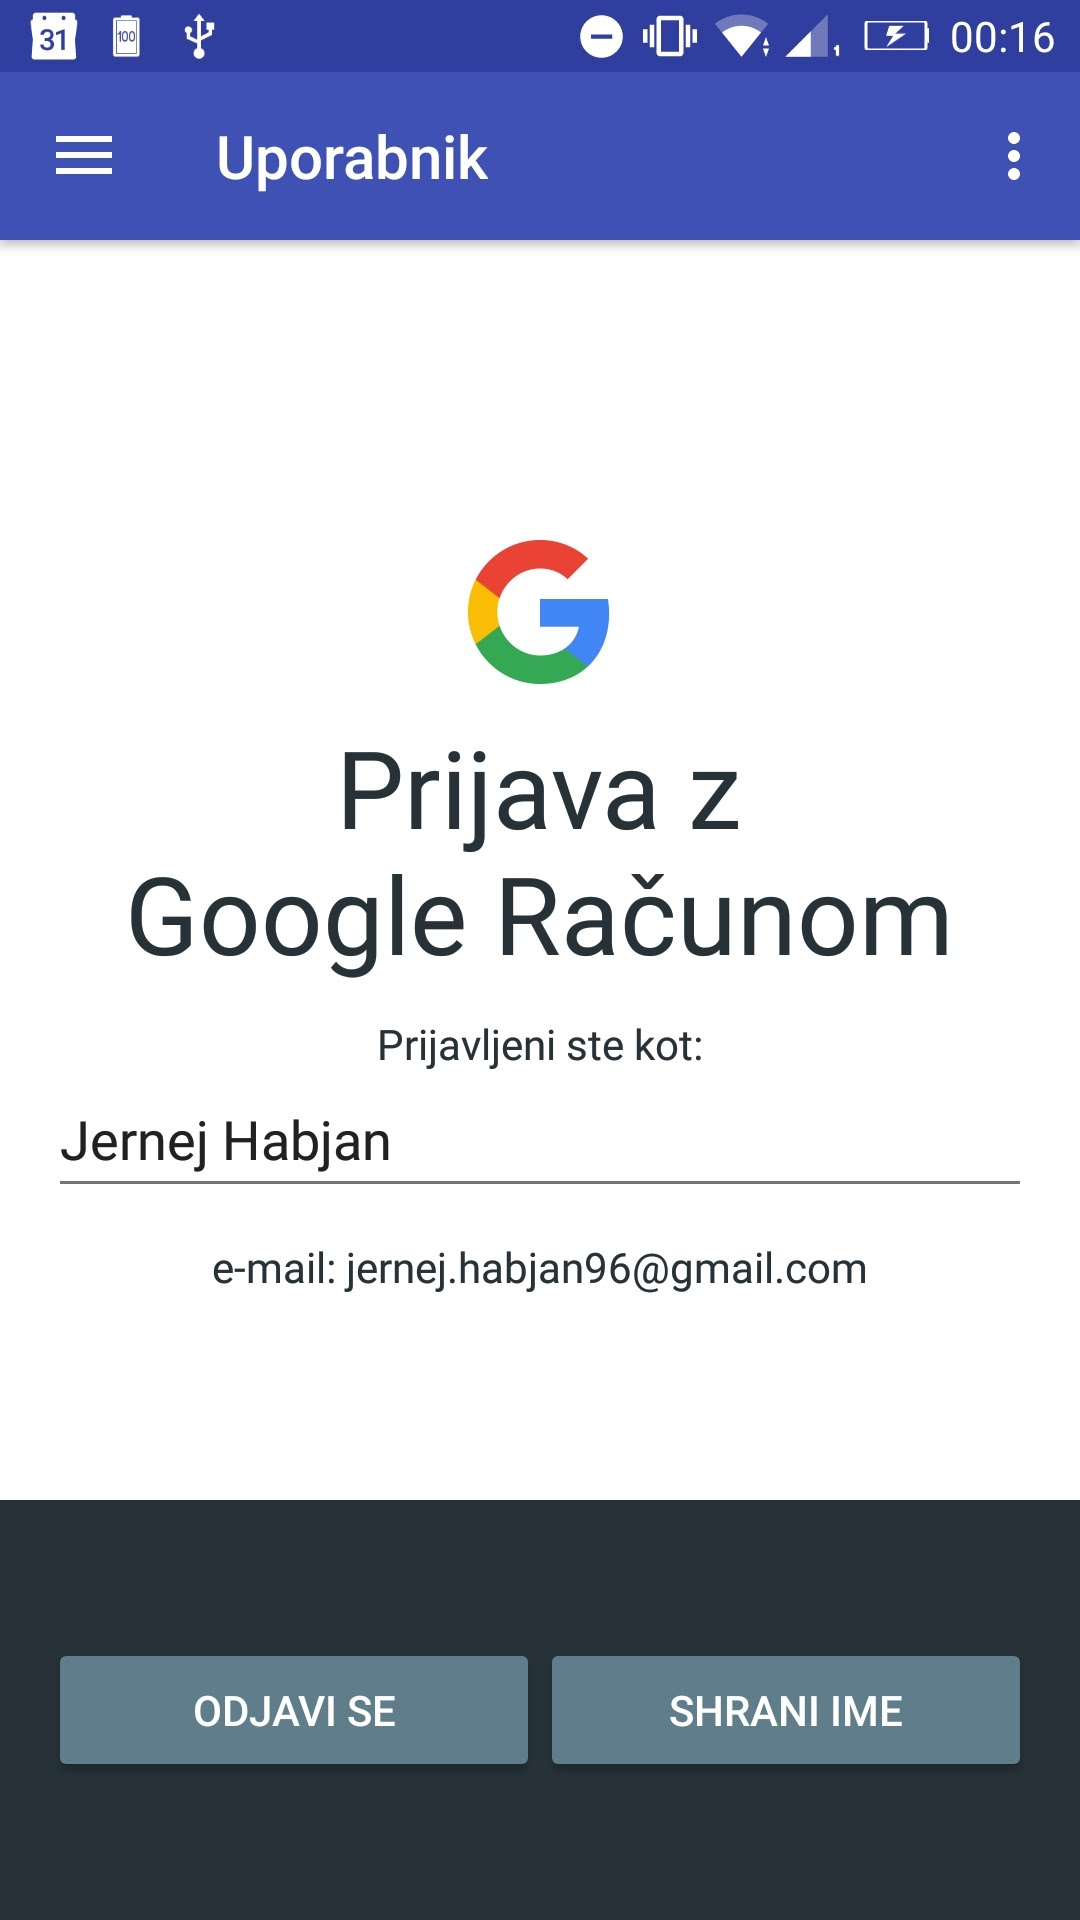
\includegraphics[width=0.2\textwidth]{loginScreen.jpg}}
\caption{Okno za prijavo uporabnika in spreminjanje imena}
\label{sl:koncept}
\end{figure}

\begin{figure}[htb]
	\centerline{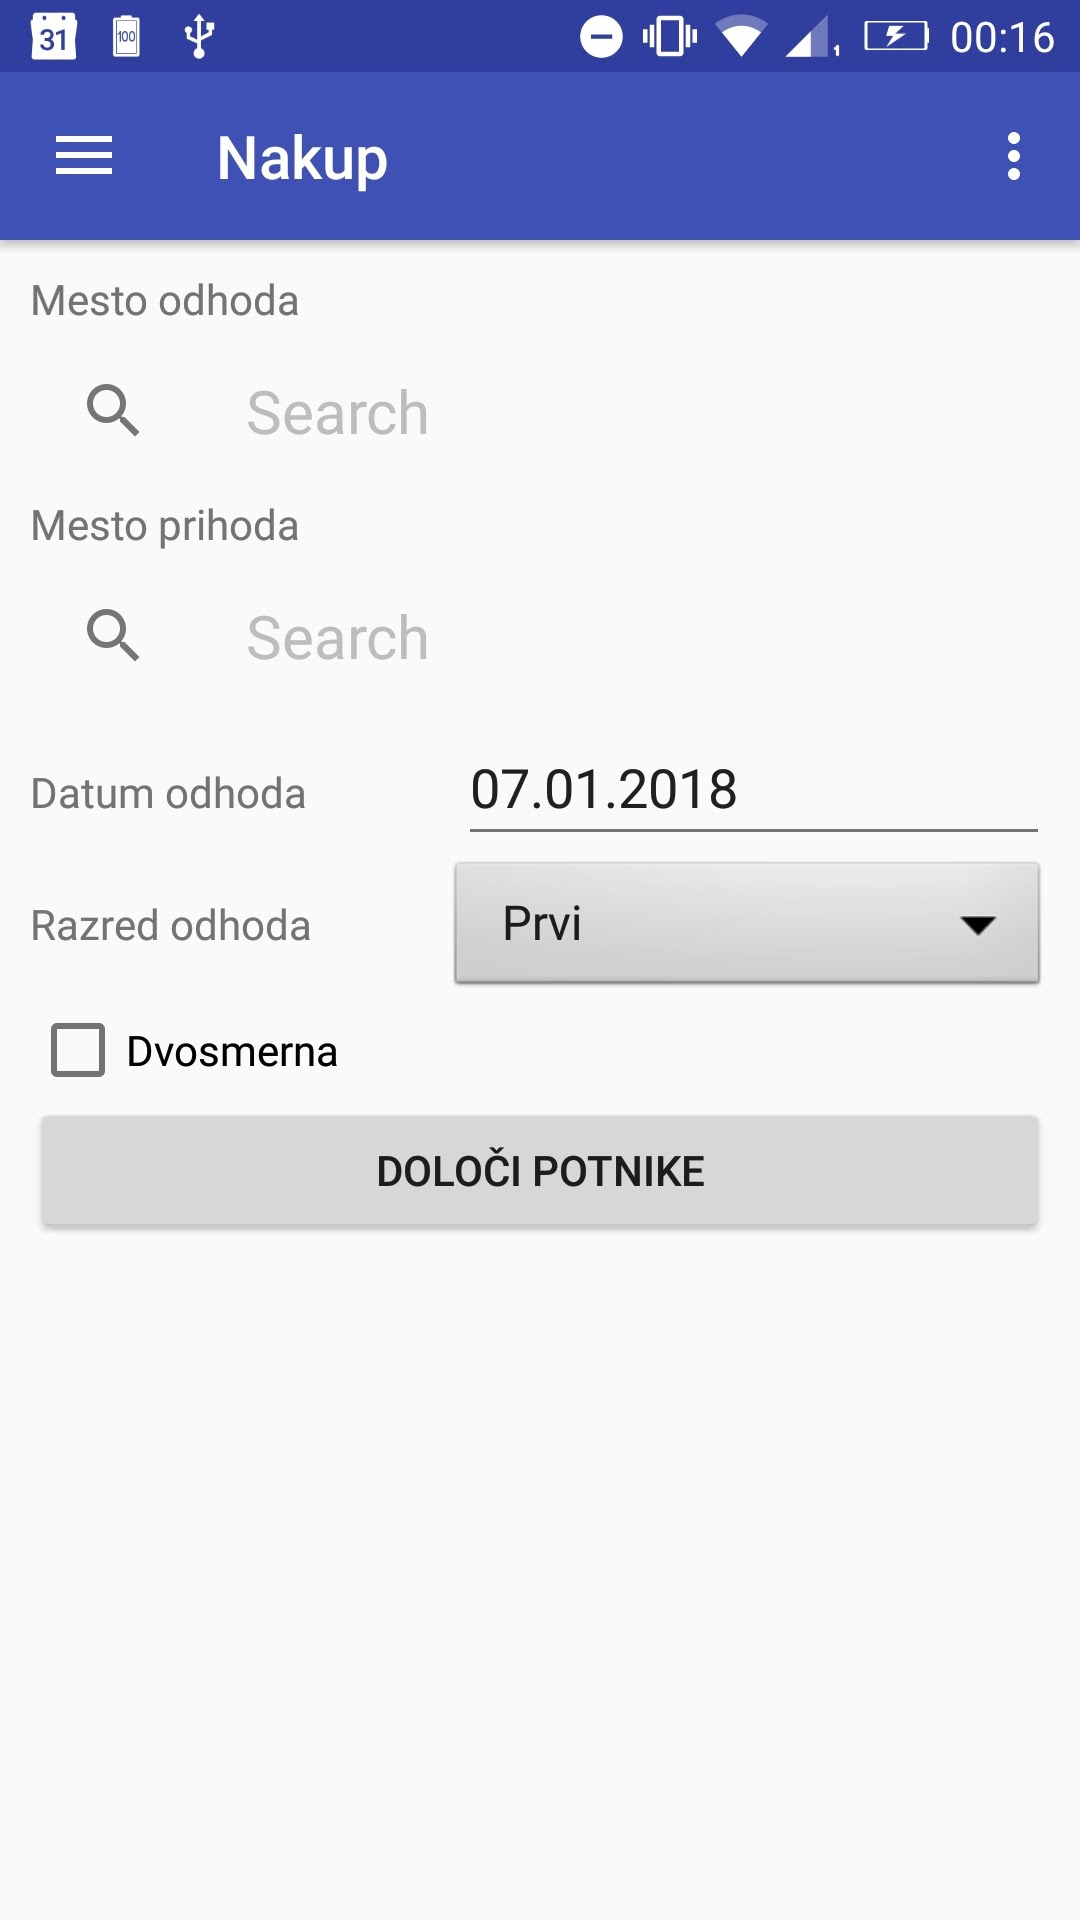
\includegraphics[width=0.2\textwidth]{nakupScreen.jpg}}
	\caption{Okno za določitev leta - vsebuje Google Autocomplete}
	\label{sl:koncept}
\end{figure}

\begin{figure}[htb]
	\centerline{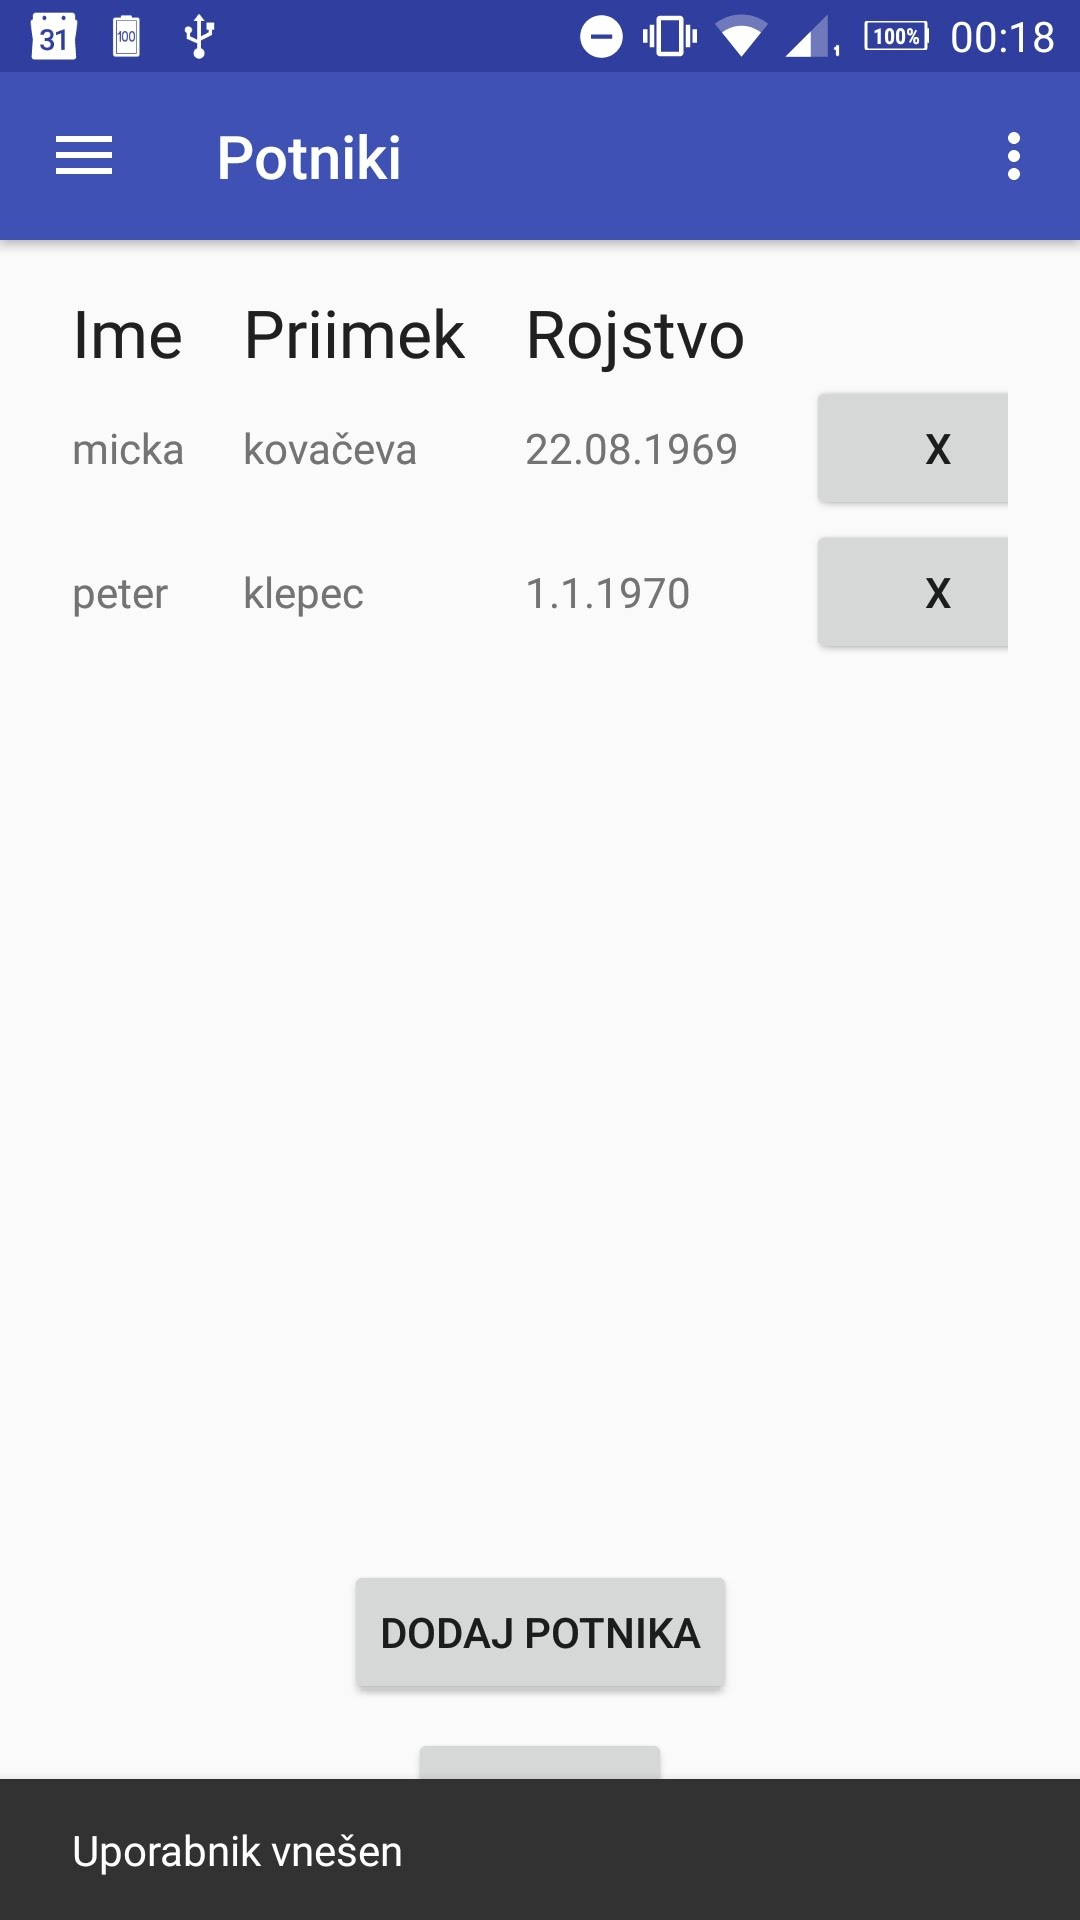
\includegraphics[width=0.2\textwidth]{potnikiScreen.jpg}}
	\caption{Prikaz vnešenih potnikov}
	\label{sl:koncept}
\end{figure}







\bibliographystyle{plain}
\bibliography{literatura}

\end{document}  




